\documentclass[12pt]{article}
\usepackage[margin=1in]{geometry}
\usepackage{amsmath}
\usepackage{listings}
\usepackage{xcolor}
\usepackage{amsthm}
\usepackage{graphicx}
\usepackage{float}
\usepackage{amssymb}


\author{ Tianran Zhang 15300180104}
\title{Project-3 Neural Network}
\lstset{
columns=fixed,
numbers=left,
frame=none,
keywordstyle=\color[RGB]{40,40,255},
numberstyle=\footnotesize\color{darkgray},
commentstyle=\it\color[RGB]{0,96,96},
stringstyle=\rmfamily\slshape\color[RGB]{128,0,0},
showstringspaces=false,
language=Matlab,
}
\begin{document}
\maketitle
\tableofcontents
\section{Neural Network}	
	In this problem we aimed to investigate handwritten digit classification. The inputs are handwritten digits, and our goal is to predict the number of the given image. Now we choose Neural Network to train the model. The basic training procedure have already given, so my work is to modify the given training procedure  and to optimize the performance.\\\\
To achieve the best test error, I do some modifications to the procedure step by step and integrate them together in the end. In the following section, I will report the modifications I made together with the best test error I have achieved. 

\subsection{Change the network structure}
In a neural network procedure, we should first set the number of layers and the hidden units in each layer. To work out the best solution, I looked up much information and find that most classification using neural network have one layer and the experienced best hidden units is (inputs number + output number)*2/3, which is equal to 178. To get the right number of units, I wrote a script named find$\_$nHidden.m(which is shown below in section 2.1) and draw a plot of validation error - units. The plots are below:
\begin{figure}[H]
	\centering
	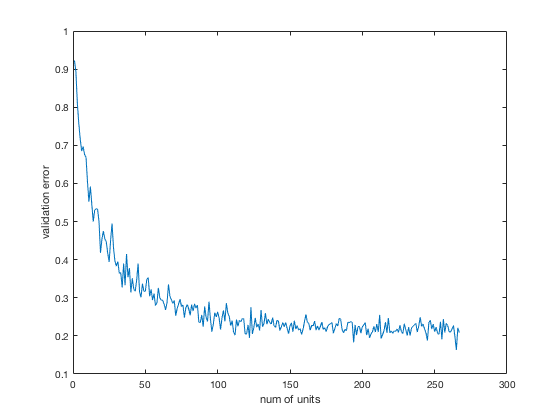
\includegraphics[width=12cm]{findnHidden.png}
	\caption{The plot of validation error - units }
\end{figure}
From the plot we could see that the validation error gets lowest when the number of units is within 100 to 250, which also contains the experienced number 178(the experienced best hidden units I have calculated before). So I choose 100 units which may save some time of the procedure. \\
\\
After setting the little change of the network structure as:
\begin{lstlisting}
nHidden = [100];
\end{lstlisting}
I trained the model for several times and got the Test error is approximately 0.24, which is half lower then the  initial Test error.\\
\subsection{Change the step-size}

In the network training procedure, the way we modify w with different step-size is very important. Choosing small step-size, we may fall into local minimum and waste much time, On the other side, choosing big step-size may be difficult for our model to get to the minimum of training error. Either big or small step-size will lead to a bad result. Now we try to deal with the problem by two ways:\\
\\
a. Modify the sequence of step-size.\\
\\
 As the sequence of step-size is : $w^{t+1} = w^t - \alpha_t\nabla f(w^t)$, where $\alpha_t$ is the learning rate (step size).  we add an item : $\beta_t(w^t - w^{t-1})$ (where $\beta_t$ = 0.9) to reduce the influence of each training on weights. So we replace the sequence of step-size by : $w^{t+1} = w^t -\alpha_t\nabla f(w^t) + \beta_t(w^t - w^{t-1})$. Now we could avoid falling into local minimum, and thus we could make the initial step-size a little bigger, and to improve the convergence.\\
\\ 
The modified part :
 \begin{lstlisting}
    i = ceil(rand*n);
    [errors(iter),  g] = funObj(w,i);

    w = w - stepSize*g + 0.9 * (w - w0);
    w0 = w;
 \end{lstlisting}
b. Use different step-size during the training. \\
\\
One way to change the step-size is to set a minStep-size and a maxStep-size. In each iteration, the step-size is : step-size = maxStep-size - $\frac{iter}{maxIter}$ (maxStep-size - minStep-size)\\
\\
The modified part :
\begin{lstlisting}
  %initialize
  stepSize = 1e-3 ;
  maxStepsize = 1e-3 * 5;
  minStepsize = maxStepsize/10;
\end{lstlisting}
For each item in the loop:
\begin{lstlisting}
    i = ceil(rand * n);
    [errors(iter),  g] = funObj(w, i);
    
    stepSize = maxStepsize - (maxStepsize - minStepsize)* iter/ maxIter;
    w = w - stepSize*g;
\end{lstlisting}
I run the model for several times and get the result that: 

If we do nothing to the step-size, the validation error convergence to 50\%;

If we do  a (modify the sequence of step-size), the validation error convergence to 32\%;

If we do  b (using different step-size), the validation error convergence to 30\%. \\
So apparently, our modification does improve the convergence.\\

\subsection{Vectorize evaluating the function}
Notice that the training procedure is quite slowly, I managed to vectorize the loss function together with the predict function by:\\
\\
a. Try to initialize the cell, vector, and matrix, and compute the values before we use them for a lot of times.\\
In the predict function:
\begin{lstlisting}
 nH = length(nHidden);
 ip = cell(1, nH);
 fp = cell(1, nH);
\end{lstlisting}
And we do the same to the loss function as well.\\
\\
b. Try to express as much as possible in terms of matrix operations.\\
In the loss function:\\
When calculating the output gradients, instead of using the loop:
\begin{lstlisting}
for c = 1:nLabels
		gOutput(:,c) = gOutput(:,c) + err(c)*fp{end}';
end
\end{lstlisting}
We can save a bunch of time by using:
\begin{lstlisting}
gOutput = gOutput + fp{end}' * err;
\end{lstlisting}
When calculating the input gradients, instead of using the loop:
\begin{lstlisting}
for c = 1:nLabels
               gInput = gInput + err(c)*X(i,:)'*(sech(ip{end}).^2.*...
                   outputWeights(:,c)');
end
\end{lstlisting}
we could use:
\begin{lstlisting}
gInput = gInput + X(i,:)' * (sech(ip{end}).^2 .* ...
                (outputWeights * err')' );   
\end{lstlisting}        
And if we have more than one hidden layers, instead of using the loop:
\begin{lstlisting}
for c = 1:nLabels
      backprop(c,:) = err(c)*(sech(ip{end}).^2.*outputWeights(:,c)');
      gHidden{end} = gHidden{end} + fp{end-1}'*backprop(c,:);
end
backprop = sum(backprop, 1);
\end{lstlisting}
We could vectorize it by : 
\begin{lstlisting}
backprop = err' * sech(ip{end}).^2 .* outputWeights';
backprop = sum(backprop,1);
gHidden{end} = gHidden{end} + fp{end-1}' * backprop;
\end{lstlisting}
After the speed up modification, I run the code and find out that the time to finish the code drops from 21s to 7s ! Which proves that the modification is effectiveness.
 
\subsection{Add l2 regrlarization}
One important modification to model training is to add a l2 regularization of the weights to the loss function, which is called $weight$ $decay$. After adding the l2 regularization, the gradients change,
\begin{align*}
E_{l2} &= E + \frac{1}{2}|weights|^2\\
grandient_{l2} &= grandient + weights\\
\end{align*}
so that we make a little change to the loss function:
\begin{align*}
gOutput_{l2} &= gOutput +outputweights\\
gHidden_{l2} &= gHidden +Hiddenweights\\
gInput_{l2} &= gIntput +inputweights
\end{align*}
Output gradients:
\begin{lstlisting}
gOutput = gOutput + fp{end}' * err + lambda * outputWeights .* ...
            [zeros(1, size(outputWeights, 2)); ...
            ones(size(outputWeights, 1)-1, ...
            size(outputWeights, 2))];
\end{lstlisting}
Input gradients:
\begin{lstlisting}
gInput = gInput + X(i,:)' * (sech(ip{end}).^2 .* ...
                (outputWeights * err')' ) + lambda * inputWeights .* ...
                [zeros(1, size(inputWeights, 2)); ...
                ones(size(inputWeights, 1)-1, ...
                size(inputWeights, 2))];  
\end{lstlisting}
Hidden gradients (if there are more than one hidden layers):
\begin{lstlisting}
backprop = err' * sech(ip{end}).^2 .* outputWeights';
            backprop = sum(backprop,1);
            gHidden{end} = gHidden{end} + fp{end-1}' * backprop + ...
                lambda * hiddenWeights{end} .* ...
                [zeros(1, size(hiddenWeights{end}, 2)); ...
                ones(size(hiddenWeights{end}, 1)-1, ...
                size(hiddenWeights{end}, 2))];
            
            % Other Hidden Layers
            for h = nH-2:-1:1
                backprop = (backprop * hiddenWeights{h+1}') .* ...
                    sech(ip{h+1}).^2;
                gHidden{h} = gHidden{h} + fp{h}'*backprop + ...
                    lambda * hiddenWeights{h} .* ...
                    [zeros(1, size(hiddenWeights{h}, 2)); ...
                    ones(size(hiddenWeights{h}, 1)-1, ...
                    size(hiddenWeights{h}, 2))];
                
            end
\end{lstlisting}
Now, is quite important to find out the best $\lambda$, I wrote a loop that make $\lambda$ ranged from 0 to 1 and find that it works better in range 0.01 to 0.06, so I adjust the loop make $\lambda$ ranged from 0.01 to 0.05. The plot is shown below:
\begin{figure}[H]
	\centering
	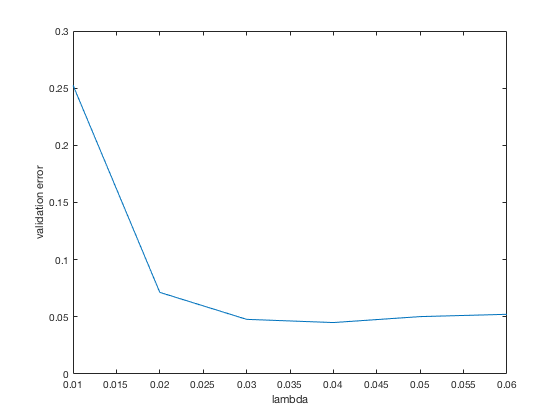
\includegraphics[width=12cm]{findLambda.png}
	\caption{The plot of validation error - lambda }
\end{figure}
From the plot we could see that $\lambda$ works best when ranged in 0.03 to 0.05, so I choose $\lambda$ = 0.03 and run the script for several times and got the Test error with final model = 0.041000.\\
\\
Except for adding a l2 regularization, I tried early stopping in the main script, which is used to stop training when the error on the validation set stops decreasing consistently for 3 times. That is : if $ validation\_error_t > validation\_error_{t-1}  > validation\_error_{t-2} $ then stop training. The modification in the loop is :
\begin{lstlisting}
	a2 = sum(yhat~=yvalid)/t;
	if (a2 > a1 )&(a1 > a0) 
            break;
        else
            a0 = a1;
            a1 = a2;
        end        
\end{lstlisting}
After running the script, I found out that the test error and time caused are both reduced largely, so I will add this method to the final script.

\subsection{Softmax layer}
Instead of using the squared error, I  use a softmax layer at the end of the network. So the 10 outputs can be interpreted as the probabilities of each class. To finish the softmax training procedure, I make some modifications to the loss function:\\
\\
a. In the last layer, $z_i = fp\{end\} outputWeights$, where i = 1...nLabels, we put them in the softmax function : $p(y_i) = \frac{exp(z_i)}{\sum_{j=1}^J exp(z_j)}$, so we calculate the probabilities in each class, and the error is $E = -logp(y_{trueLabel})$:
\begin{lstlisting}
    yhat1 = exp(fp{end}*outputWeights);
    yhat = yhat1/sum(yhat1);
    [~, y_true] = max(y(i, :));
    yhat_true = yhat(y_true);
    err = -log(yhat_true);
    f=f + err;
\end{lstlisting}
b. Since we changed the output numbers, the gradients changed, too. So we made the calculation by :
\begin{align*}
\frac{\partial{E}}{\partial{outputWeights}} 
& = \frac{\partial{E}}{\partial{P(y_{trueLabel})}} \frac{{\partial{P(y_{trueLabel})}}}{\partial{z}} \frac{\partial{z}}{\partial{outputWeights}}\\
& = -\frac{1}{p(y_{trueLabel})} \frac{{\partial{P(y_{trueLabel})}}}{\partial{z}}  fp\{end\}\\
%& = fp\{end\}' (1-p(y_{trueLabel}))	\\					%DSGF
\\
\frac{\partial{E}}{\partial{inputWeights}}
&= \frac{\partial{E}}{\partial{P(y_{trueLabel})}} \frac{{\partial{P(y_{trueLabel})}}}{\partial{z}} \frac{\partial{z}}{\partial{fp\{1\}}} \frac{\partial{fp\{1\}}}{\partial{inputWeights}}\\
& = -\frac{1}{p(y_{trueLabel})} \frac{{\partial{P(y_{trueLabel})}}}{\partial{z}} outputWeights(:) X(i, :)\\
\end{align*} 
I applied this on matlab:
\begin{lstlisting}
gOutput = gOutput - fp{end}' * (1 - yhat_true) * (y(i,:)==1);

gInput = gInput - (1 - yhat_true) * X(i,:)' * ...
( sech(ip{end}).^2 .* outputWeights(:, y(i,:)==1)' );
\end{lstlisting}
Then I run the script (which is shown below in Sec.3) for several times and got the result that the validation error is convergence to 18\%, so I will add this method to the final script.

\subsection{Add bias in each layer}
Instead of just having a bias variable at the beginning, I made the last units of each layer a constant, so that each layer has a bias.\\
\\
Since I made the last units of each layer a constant, the weights for each layers should be redistributed as:
\begin{lstlisting}
inputWeights = reshape(w(1:nVars*(nHidden(1)-1)), nVars, nHidden(1)-1);
offset = nVars * (nHidden(1)-1);
for h = 2:nH
	 hiddenWeights{h-1} = reshape(...
            w(offset+1 : offset+nHidden(h-1)*(nH idden(h)-1)),...
            nHidden(h-1) , nHidden(h)-1);	
	 offset = offset + nHidden(h-1)*(nHidden(h)-1);
end
outputWeights = w(offset+1:offset+nHidden(end)*nLabels);
outputWeights = reshape(outputWeights, nHidden(end), nLabels);
\end{lstlisting}
And since each layers have one units remains const, we should calculate the gradients and backprop without the consts' influence, that is:
\begin{lstlisting}
% Output Weights
gOutput = gOutput + fp{end}' * err;

if nH > 1
	% Last Layer of Hidden Weights
	backprop = err' * sech(ip{end}).^2 .* outputWeights';
	backprop = sum(backprop,1);
	g1 = fp{end-1}' * backprop;
	gHidden{end} = gHidden{end} + g1(: , 1: nHidden(end)-1);

	% Other Hidden Layers
	for h = nH-2 : -1 : 1
			g1 = (backprop * hiddenWeights{h+1}') .* ...
			sech(ip{h+1}).^2;
			backprop = g1(:, 1: nHidden(h)-1);
			gHidden{h} = gHidden{h} + fp{h}'*backprop;
	end

	% Input Weights
	g1 = (backprop(:, 1:nHidden(2)-1)*hiddenWeights{1}') .* ...
		sech(ip{1}).^2;
	backprop = g1(:, 1:nHidden(1)-1);
	gInput = gInput + X(i,:)'*backprop;
else
	% Input Weights
	gx = X(i,:)' * (sech(ip{end}).^2 .* ...
			(outputWeights * err')' );
	gInput = gInput + gx(: , 1: nHidden(1)-1);
end
\end{lstlisting}
When we do the prediction of valid data or test data, we shall also make a little change:
\begin{lstlisting}
for i = 1:nInstances
    ip{1} = [X(i,:)*inputWeights, 1];
    fp{1} = tanh(ip{1});
    for h = 2:nH
        ip{h} = [fp{h-1}*hiddenWeights{h-1}, 1];
        fp{h} = tanh(ip{h});
    end
    y(i,:) = fp{end}*outputWeights;
end
[~, y] = max(y,[],2);
\end{lstlisting}

\subsection{Implement 'dropout'}
In this section, we randomly dropped out some hidden units with probability p during the training. This is the dropout method. When we choose p = 0.5 as a commen choice, we randomly dropped half units, which is a good way to prevent over-fitting.\\
We used to train the netural network with:
\begin{align*}
ip(l+1) = w^{l+1}y^l\\
fp(l+1) = tanh(ip(l+1))
\end{align*}
But after we adapt dropout method, the calculation formula comes to :
\begin{align*}
r_j^l \sim Bernoulli(p)\\
\tilde y^l = r^l * y^l\\
ip(l+1) = w^{l+1}\tilde y^l\\
fp(l+1) = tanh(ip(l+1))
\end{align*}
I applied it on the loss function:
\begin{lstlisting}
    p{1} = [rand(1, nHidden(1))>0.5];
   
    ip{1} = X(i,:) * inputWeights .* p{1};
    fp{1} = tanh(ip{1});
    for h = 2:nH
        p{h} = [rand(1, nHidden(h))>0.5];
        ip{h} = fp{h-1} * hiddenWeights{h-1} .* p{h};
        fp{h} = tanh(ip{h});
    end
\end{lstlisting}
When we calculate the gradients, we should still drop out the chosen units:
\begin{lstlisting}
gOutput = (gOutput + fp{end}' * err) .* repmat(p{end}', 1, nLabels);
        
if nH > 1
   % Last Layer of Hidden Weights
    backprop = err' * sech(ip{end}).^2 .* outputWeights';
    backprop = sum(backprop,1);
    gHidden{end} = (gHidden{end} + fp{end-1}' * backprop) .* ...
    repmat(p{end-1}', 1, length(p{end})) .* ...
    repmat(p{end}, length(p{end-1}), 1);
            
     % Other Hidden Layers
     for h = nH-2:-1:1
          backprop = (backprop * hiddenWeights{h+1}') .* ...
                    sech(ip{h+1}).^2;
          gHidden{h} = (gHidden{h} + fp{h}'*backprop) .* ...
                    (p{h}'*p{h+1});
      end
            
      % Input Weights
      backprop = (backprop*hiddenWeights{1}').*sech(ip{1}).^2;
      gInput = (gInput + X(i,:)'*backprop) .* repmat(p{1}, nVars, 1);
else
      % Input Weights
      gInput = gInput + X(i,:)' * (sech(ip{end}).^2 .* ...
                (outputWeights * err')');
           
      gInput = gInput .* repmat(p{1}, nVars, 1);
\end{lstlisting}
Now I run the main script and find out that the validation convergence to 22$\%$ with the convergence speed improved largely. So I will add this method into the final script.

\subsection{'fine-tuning'}
We do 'fine-tuning' to the last layer : Fix the parameters of all the layers except the last one, and solve for the outputWeights exactly as a convex optimization problem :
\begin{align*}
fp\{end\} outputWeights &= y_i\\
fp\{end\}' fp\{end\} outputWeights &=fp\{end\}' y_i\\
outputWeights &= (fp\{end\}' fp\{end\})^{-1} fp\{end\}' y_i
\end{align*}
I applied it on Matlab:
\begin{lstlisting}
outputWeights = pinv(fp{end}' * fp{end}) * fp{end}' * y(i,:);
\end{lstlisting}
After working out the exact outputWeights, we use it to form the new weights:
\begin{lstlisting}
w(offset+1:offset+nHidden(end)*nLabels) = outputWeights(:);
\end{lstlisting}
Through the new weights to calculate the gradients of weights as we have done before.\\
I run the script for several times, the results doesn't seem well:
\begin{lstlisting}
>> MLP8
Training iteration = 0, validation error = 0.901200
Training iteration = 5000, validation error = 0.856600
Training iteration = 10000, validation error = 0.851400
Training iteration = 15000, validation error = 0.912400
Training iteration = 20000, validation error = 0.919000
Training iteration = 25000, validation error = 0.865400
Training iteration = 30000, validation error = 0.864000
Training iteration = 35000, validation error = 0.892600
Training iteration = 40000, validation error = 0.907600
Training iteration = 45000, validation error = 0.878200
Training iteration = 50000, validation error = 0.863600
Training iteration = 55000, validation error = 0.890200
Training iteration = 60000, validation error = 0.878200
Training iteration = 65000, validation error = 0.905600
Training iteration = 70000, validation error = 0.849800
Training iteration = 75000, validation error = 0.853800
Training iteration = 80000, validation error = 0.879800
Training iteration = 85000, validation error = 0.866000
Training iteration = 90000, validation error = 0.894800
Training iteration = 95000, validation error = 0.882200
Elapsed time is 16.472326 seconds.
Test error with final model = 0.904000
\end{lstlisting}
It seems that the validation error doesn't change much. This is because when the outputWeights being exactly the matrix which $fp\{end\} outputWeights = y_i$, then the error : $E = y_i - fp\{end\} outputWeights$, which is approximately 0. So when we calculate the gradients, they are approximately equal to 0, too. So, during the training procedure, we don't change the weights and thus lead to its bad performance. And I won't add this method to my final script.

\subsection{Create more training examples}
Since the handwriting could be less precise (too big or too small, rotate clockwise or anti-clockwise, etc.) So we artificially creat more training examples by applying small transforations (like rotations and resizing, etc.) to the original images :
\begin{lstlisting}
for i = 1:size(X,1)
	X1 = imrotate(reshape(X(i,:),16,16), 5, 'crop');
	X_clock(i,:) = X1(:);
	X1 = imrotate(reshape(X(i,:),16,16), -5, 'crop');
	X_anticlock(i,:) = X1(:);
	X1 = imresize(reshape(X(i,:),16,16), 1.1, 'OutputSize', [16,16]);
	X_big(i,:) = X1(:);
	X1 = imresize(reshape(X(i,:),16,16), 0.9, 'OutputSize', [16,16]);
	X_small(i,:) = X1(:);
end

X = [X; X_clock; X_anticlock; X_big; X_small];
y = repmat(y,5,1);
\end{lstlisting}
After create the new training set (X, y), we train our model as before with the new training set and find that the validation error convergent to 20$\%$. The method works better when we got less dataset, but I think that is because our training model is not big enough. This method will work better when the training data is more large and more chaos, so I will not use it in the final script.

\subsection{2D convolutional layer}
In this section, we replace the first layer of the network with a 2D convolutional layer and train the model by the following step:\\
a. Reshape the USPS images back to their original 16 by 16 format:
\begin{lstlisting}
[X,mu,sigma] = standardizeCols(X);
X = reshape(X',16,16,n);

Xvalid = standardizeCols(Xvalid,mu,sigma);
Xvalid = reshape(Xvalid',16,16,t);

Xtest = standardizeCols(Xtest,mu,sigma);
Xtest = reshape(Xtest',16,16,t2);
\end{lstlisting}
b. For each iteration, we randomly choose i from 1 to n(number of trainning data), and then finish the convolution layer c1 use the $conv2$ function:
\begin{lstlisting}
i = ceil(rand*n);
X1 = X(:,:,i);

c1 = zeros(12,12,nConv);
for k = 1:nConv
	c1(:,:,k) = conv2(X1,rot90(cWeights(:,:,k),2),'valid');
	c1(:,:,k) = tanh(c1(:,:,k) + cBias(1,k));
end
\end{lstlisting}
c. Now we finish the full-connected layer: put the convolution layer c1 into norml 16 x 16 format and make the connection to the hidden layer:
\begin{lstlisting}
for n = 1:nHidden
	count = 0;
	for m = 1:nConv
		count = count + c1(:,:,m) * hiddenWeights(m,n);
	end
	e(:,:,n) = count;
	f1(:,:,n) = conv2(e(:,:,n), ...
	rot90(fWeights(:,:,n),2), 'valid');
end 

for h = 1:nLabels
	output(1,h) = exp( f0*outputWeights(:,h) ) / ...
	sum( exp(f0*outputWeights) );
end
\end{lstlisting}
c. Using softmax method to generate the output layer because we don't have the exact prediction to each label :
\begin{lstlisting}
output = zeros(1, nLabels);
for h = 1:nLabels
	output(1,h) = exp( f0*outputWeights(:,h) ) / ...
	sum( exp(f0*outputWeights) );
end
\end{lstlisting}
d. To updating the weights and bias, I wrote a function named $ConvUpdate$ and the predict function named $ConvPredict$ is shown in Sec.3:
\begin{lstlisting}
    % Update weights, kernels and bias.
    [cWeights, fWeights, hiddenWeights, outputWeights, cBias, fBias] = ...
        WechatCNN_update(stepSize, y(i), X1, c1, f0, ...
        e, output, cWeights, fWeights, hiddenWeights, ...
        outputWeights, cBias, fBias);
\end{lstlisting}

After running the script, I got the result that validation error convergence to 25$\%$. For the training procedure is too slowly, I just set the maxIter = 10000, and The result seems not bad, but it still causes a lot of time, so I choose not use this method  in my final script.

\section{Final script}
After finishing all the 10 questions, I did all the following adjustment to my final script:\\
a. I choose nHidden=[100];\\
b. Modify the sequence of step-size by  $w^{t+1} = w^t -\alpha_t\nabla f(w^t) + \beta_t(w^t - w^{t-1})$, where $\beta_t = 0.9$\\
c. Vectorize the evaluating the function to speed up the training;\\
d. Add a l2 regularization $\lambda = 0.03$;\\
e. Use a softmax layer at the end of the network;.
Run the final script for several times, The test error is approximately 6$\%$.
The final script is shown in Sec.3.
\section{Matlab Code}
\subsection{LossSoftmax}
\begin{lstlisting}
function [f,g] = LossSoftmax(w,X,y,nHidden,nLabels)
% g : the new weights
% f : the gradient
%
% Tianran Zhang Dec.6th

[nInstances,nVars] = size(X);
nH = length(nHidden);

% Form Weights
inputWeights = reshape(w(1:nVars*nHidden(1)),nVars,nHidden(1));
offset = nVars*nHidden(1);
for h = 2:length(nHidden)
    hiddenWeights{h-1} = reshape(w(offset+1 : offset+nHidden(h-1) * ...
        nHidden(h)), nHidden(h-1), nHidden(h));
    offset = offset + nHidden(h-1) * nHidden(h);
end
outputWeights = w(offset+1 : offset+nHidden(end)*nLabels);
outputWeights = reshape(outputWeights, nHidden(end), nLabels);

f = 0;
ip = cell(1, nH);
fp = cell(1, nH);
if nargout > 1
    gInput = zeros(size(inputWeights));
    gHidden = cell(1, nH-1);
    for h = 2:nH
        gHidden{h-1} = zeros(size(hiddenWeights{h-1}));
    end
    gOutput = zeros(size(outputWeights));
end

% Compute Output
for i = 1:nInstances
    ip{1} = X(i,:) * inputWeights;
    fp{1} = tanh(ip{1});
    for h = 2:length(nHidden)
        ip{h} = fp{h-1} * hiddenWeights{h-1};
        fp{h} = tanh(ip{h});
    end
    
    yhat1 = exp(fp{end}*outputWeights);
    yhat = yhat1/sum(yhat1);
    [~, y_true] = max(y(i, :));
    yhat_true = yhat(y_true);
    err = -log(yhat_true);
    f=f + err;
    
    if nargout > 1
        
        % Output Weights
        gOutput = gOutput - fp{end}' * (1 - yhat_true) * (y(i,:)==1);%
        if nH > 1
            % Last Layer of Hidden Weights
            backprop = err' * sech(ip{end}).^2 .* outputWeights';
            gHidden{end} = gHidden{end} + fp{end-1}' * sum(backprop,1);            
            backprop = sum(backprop,1);
        
            
            % Other Hidden Layers
            for h = nH-2:-1:1
                backprop = (backprop*hiddenWeights{h+1}') .* ...
                    sech(ip{h+1}).^2;
                gHidden{h} = gHidden{h} + fp{h}' * backprop;
            end
            
            % Input Weights
            backprop = (backprop*hiddenWeights{1}') .* sech(ip{1}).^2;
            gInput = gInput + X(i,:)' * backprop;
        else
            % Input Weights
            gInput = gInput - (1 - yhat_true) * X(i,:)' * ...
                ( sech(ip{end}).^2 .* outputWeights(:, y(i,:)==1)' );
            
        end
    end
end

% Put Gradient into vector
if nargout > 1
    g = zeros(size(w));
    g(1:nVars*nHidden(1)) = gInput(:);
    offset = nVars*nHidden(1);
    for h = 2:nH
        g(offset+1:offset+nHidden(h-1)*nHidden(h)) = gHidden{h-1};
        offset = offset+nHidden(h-1)*nHidden(h);
    end
    g(offset+1:offset+nHidden(end)*nLabels) = gOutput(:);
end
\end{lstlisting}

\subsection{PredictSoftmax}
\begin{lstlisting}
%Tianran Zhang Dec.6th

function [y] = MLPclassificationPredict(w,X,nHidden,nLabels)
[nInstances,nVars] = size(X);

% Form Weights
inputWeights = reshape(w(1:nVars*nHidden(1)),nVars,nHidden(1));
offset = nVars*nHidden(1);

for h = 2:length(nHidden)
  hiddenWeights{h-1} = reshape(w(offset+1 : offset + ...
      nHidden(h-1)*nHidden(h)),nHidden(h-1),nHidden(h));
  offset = offset+nHidden(h-1)*nHidden(h);
end

outputWeights = w(offset+1:offset+nHidden(end)*nLabels);
outputWeights = reshape(outputWeights,nHidden(end),nLabels);

% Compute Output
y = zeros(nInstances, 1);
for i = 1:nInstances
    ip{1} = X(i,:)*inputWeights;
    fp{1} = tanh(ip{1});
    for h = 2:length(nHidden)
        ip{h} = fp{h-1}*hiddenWeights{h-1};
        fp{h} = tanh(ip{h});
    end
    yhat1 = exp(fp{end}*outputWeights);
    yhat(i,:) = yhat1/sum(yhat1);
end
[v,y] = max(yhat,[],2);
\end{lstlisting}
\subsection{ConvPredict}
\begin{lstlisting}
function [yhat] = ConvPredict(X, cWeights, fWeights, hiddenWeights, ...
    outputWeights, cBias, fBias)

nInstances = size(X, 3);
yhat = zeros(nInstances, 1);
nConv = size(cWeights, 3);
[nHidden, nLabels] = size(outputWeights);
c1 = size(X,1) - size(cWeights,1) + 1;
c2 = size(X,2) - size(cWeights,2) + 1;

for i = 1:nInstances
    train_data = X(:,:,i);
    
    c0 = zeros(c1, c2, nConv);
    for k = 1:nConv
        c0(:,:,k) = conv2(train_data,rot90(cWeights(:,:,k),2),'valid');
        c0(:,:,k) = tanh(c0(:,:,k) + cBias(1,k));
    end
    
    [f1,~] = conv(c0, fWeights, hiddenWeights);
    f = zeros(1, nHidden);
    for h = 1:nHidden
        f(1,h) = tanh(f1(:,:,h) + fBias(1,h));
    end
    
    output = zeros(1, nLabels);
    for h = 1:nLabels
        output(1,h) = exp( f * outputWeights(:,h) ) / ...
            sum( exp(f * outputWeights) );
    end
    [~, yhat(i)] = max(output);
end

end
\end{lstlisting}

\subsection{final$\_$MLP}
\begin{lstlisting}
%Final script
%
% Tianran Zhang, Dec. 5, 2017.

load digits.mat
[n,d] = size(X);
nLabels = max(y);
yExpanded = linearInd2Binary(y,nLabels);
t = size(Xvalid,1);
t2 = size(Xtest,1);

% Standardize columns and add bias
[X,mu,sigma] = standardizeCols(X);
X = [ones(n,1) X];
d = d + 1;

% Make sure to apply the same transformation to the validation/test data
Xvalid = standardizeCols(Xvalid,mu,sigma);
Xvalid = [ones(t,1) Xvalid];
Xtest = standardizeCols(Xtest,mu,sigma);
Xtest = [ones(t2,1) Xtest];

% Choose network structure
nHidden = [100];

% Count number of parameters and initialize weights 'w'
nParams = d*nHidden(1);
for h = 2:length(nHidden)
    nParams = nParams+nHidden(h-1)*nHidden(h);
end
nParams = nParams+nHidden(end)*nLabels;
maxIter = 100000;
w = randn(nParams,1);

% Train with stochastic gradient
stepSize = 1e-3;

funObj = @(w,i)Loss_final(w,X(i,:),yExpanded(i,:),nHidden,nLabels, 0.03);

tic;
w0 = 0;
a0 = 1;
a1 = 1;
for iter = 1:maxIter    
  if mod(iter-1,round(maxIter/20)) == 0
     yhat = Predict5(w,Xvalid,nHidden,nLabels);
     a2 = sum(yhat~=yvalid)/t;
     fprintf('Training iteration = %d, validation error = %f\n',iter-1, a2);
      
     %%early stop       
     if (a2 > a1 )&(a1 > a0)           
       break;
     else
         a0 = a1;
         a1 = a2;
     end        
 end
    
    i = ceil(rand*n);
    [~, g] = funObj(w,i); 
    w = w - stepSize*g + 0.9 * (w - w0);
    w0 = w;
end
toc;

% Evaluate test error
yhat = Predict5(w, Xtest, nHidden, nLabels);
fprintf('Test error with final model = %f\n',sum(yhat~=ytest)/t2);

\end{lstlisting}
\subsection{Loss$\_$final}
\begin{lstlisting}
function [f,g] = Loss_final(w,X,y,nHidden,nLabels, lambda)
% Tianran Zhang, Dec. 7th
% g : the new weights
% f : the gradient

[nInstances,nVars] = size(X);
nH = length(nHidden);

% Form Weights
inputWeights = reshape(w(1:nVars*nHidden(1)),nVars,nHidden(1));
offset = nVars*nHidden(1);
for h = 2:length(nHidden)
    hiddenWeights{h-1} = reshape(w(offset+1 : offset+nHidden(h-1) * ...
        nHidden(h)), nHidden(h-1), nHidden(h));
    offset = offset + nHidden(h-1) * nHidden(h);
end
outputWeights = w(offset+1 : offset+nHidden(end)*nLabels);
outputWeights = reshape(outputWeights, nHidden(end), nLabels);

f = 0;
ip = cell(1, nH);
fp = cell(1, nH);
if nargout > 1
    gInput = zeros(size(inputWeights));
    gHidden = cell(1, nH-1);
    for h = 2:nH
        gHidden{h-1} = zeros(size(hiddenWeights{h-1}));
    end
    gOutput = zeros(size(outputWeights));
end

% Compute Output
for i = 1:nInstances
    ip{1} = X(i,:) * inputWeights;
    fp{1} = tanh(ip{1});
    for h = 2:length(nHidden)
        ip{h} = fp{h-1} * hiddenWeights{h-1};
        fp{h} = tanh(ip{h});
    end
    
    yhat1 = exp(fp{end}*outputWeights);
    yhat = yhat1/sum(yhat1);
    [~, y_true] = max(y(i, :));
    yhat_true = yhat(y_true);
    err = -log(yhat_true);
    f=f + err;
    
    if nargout > 1
        
        % Output Weights
        gOutput = gOutput - fp{end}' * (1 - yhat_true) * (y(i,:)==1) + ...
            lambda * outputWeights .* ...
            [zeros(1, size(outputWeights, 2)); ...
            ones(size(outputWeights, 1)-1, size(outputWeights, 2))];      
       
        if nH > 1
            % Last Layer of Hidden Weights
            backprop = err' * sech(ip{end}).^2 .* outputWeights';
            gHidden{end} = gHidden{end} + fp{end-1}' * sum(backprop,1);
            
            backprop = sum(backprop,1);
         %   gHidden{end} = gHidden{end} + fp{end-1}' * backprop;
            
            % Other Hidden Layers
            for h = nH-2:-1:1
                backprop = (backprop*hiddenWeights{h+1}') .* ...
                    sech(ip{h+1}).^2;
                gHidden{h} = gHidden{h} + fp{h}' * backprop;
            end
            
            % Input Weights
            backprop = (backprop*hiddenWeights{1}') .* sech(ip{1}).^2;
            gInput = gInput + X(i,:)' * backprop;
        else
            % Input Weights
            gInput = gInput - (1 - yhat_true) * X(i,:)' * ...
                ( sech(ip{end}).^2 .* outputWeights(:, y(i,:)==1)')+...
                lambda * inputWeights .* ...
                [zeros(1, size(inputWeights, 2)); ...
                ones(size(inputWeights, 1)-1, size(inputWeights, 2))];
            
        end
    end
end

% Put Gradient into vector
if nargout > 1
    g = zeros(size(w));
    g(1:nVars*nHidden(1)) = gInput(:);
    offset = nVars*nHidden(1);
    for h = 2:nH
        g(offset+1:offset+nHidden(h-1)*nHidden(h)) = gHidden{h-1};
        offset = offset+nHidden(h-1)*nHidden(h);
    end
    g(offset+1:offset+nHidden(end)*nLabels) = gOutput(:);
end
\end{lstlisting}
\subsection{Predict$\_$final}
\begin{lstlisting}
function [y] = Predict_final(w,X,nHidden,nLabels)
% Tianran Zhang Dec. 8th
[nInstances,nVars] = size(X);

% Form Weights
inputWeights = reshape(w(1:nVars*nHidden(1)),nVars,nHidden(1));
offset = nVars*nHidden(1);

for h = 2:length(nHidden)
  hiddenWeights{h-1} = reshape(w(offset+1 : offset + ...
      nHidden(h-1)*nHidden(h)),nHidden(h-1),nHidden(h));
  offset = offset+nHidden(h-1)*nHidden(h);
end

outputWeights = w(offset+1:offset+nHidden(end)*nLabels);
outputWeights = reshape(outputWeights,nHidden(end),nLabels);

% Compute Output
y = zeros(nInstances, 1);
for i = 1:nInstances
    ip{1} = X(i,:)*inputWeights;
    fp{1} = tanh(ip{1});
    for h = 2:length(nHidden)
        ip{h} = fp{h-1}*hiddenWeights{h-1};
        fp{h} = tanh(ip{h});
    end
    yhat1 = exp(fp{end}*outputWeights);
    yhat(i,:) = yhat1/sum(yhat1);
   % [~, y(i)] = max(yhat(i, :));
end
[v,y] = max(yhat,[],2);

\end{lstlisting}
\end{document}














